\section{Sistema B – Controlo de Climatização}

É requisitado que dada uma temperatura, obtida através do sensor DHT, e um intervalo de temperaturas máxima e mínima (25 e 20, respetivamente), o sistema seja capaz de manter uma temperatura ambiente controlada com recurso a uma ventoínha.

Como tal, sempre que a temperatura ultrapassar a temperatura \textbf{máxima}, a ventoínha deve ser acionada até que a temperatura registada seja inferior à temperatura \textbf{mínima}.

\begin{figure}[H]
    \centering
    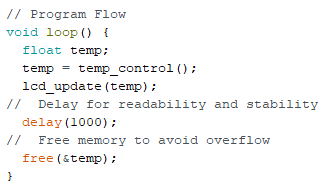
\includegraphics{images/codigo/sisB_loop.png}
    \selectlanguage{portuguese}\caption{Função loop()}
\end{figure}

Esta função controla o `flow' do Programa. Como se pode verificar, está definido o controlo de temperatura seguido da atualização do LCD. Por fim, um delay para estabilidade das leituras e apresentação do LCD.

\begin{figure}[H]
    \centering
    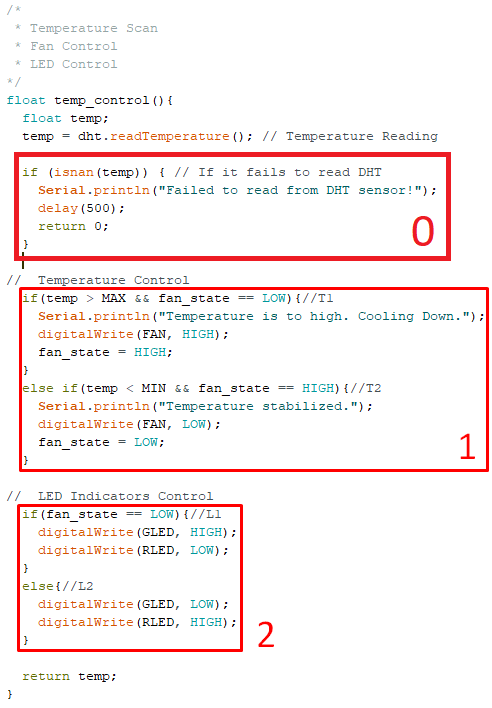
\includegraphics[scale=0.5]{images/codigo/sisB_temp.png}
    \selectlanguage{portuguese}\caption{Função temp\_control()}
\end{figure}

\begin{enumerate}
  \setcounter{enumi}{-1}
    \item Falha de leitura da temperatura pelo sensor DHT
    \item Definição do estado da ventoínha em função da temperatura observada.
    \begin{itemize}
        \item Transição entre estado \textbf{estável} e \textbf{arrefecimento}
        \item Transição entre estado \textbf{arrefecimento} e \textbf{estável}
    \end{itemize}
    \item Definição do estado do sistema utilizando LEDs em função do estado da ventoínha.
\end{enumerate}

\begin{figure}[H]
    \centering
    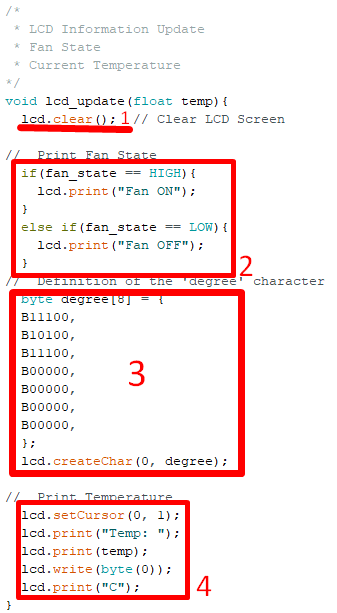
\includegraphics[scale=0.5]{images/codigo/sisB_lcd.png}
    \selectlanguage{portuguese}\caption{Função lcd\_update()}
\end{figure}

\begin{enumerate}
    \item Limpeza do ecrã do LCD e consequente reposiçãodo cursor.
    \item Apresentação do estado atual da Ventoínha.
    \item Definição do caracter `$^{o}$'.
    \item Apresentação da última temperatura lida.
\end{enumerate}